\chapter{Methods}
\section{Semantic segmentation}
\subsection{DeepLab}
One of the challenges in semantic segmentation using standard CNNs is that as the input feature map goes through the network
it gets smaller and the information about objects of a smaller scale can be lost.
DeepLab family introduces atrous convolutions that extract more dense features
which help to preserve the object's information. Compared to standard convolutions, atrous convolutions have an additional parameter, atrous
rate, which is the stride at which the input is sampled (Figure~\ref*{fig:aconv} a).
The atrous convolution is used in the last few blocks on features that were extracted from the backbone network (e.g. ResNet~\cite{he2016deep}).

\begin{wrapfigure}{r}{0.5\textwidth}
  \centering
  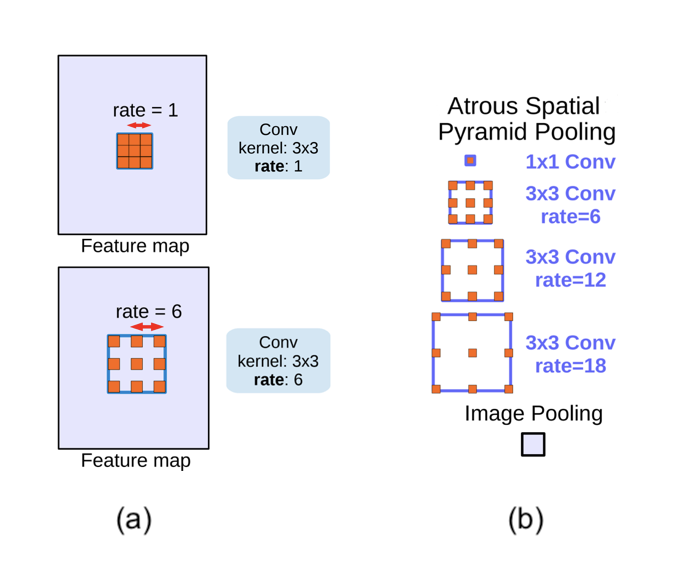
\includegraphics[width=0.5\textwidth]{figures/conv_aspp.png} %choose your uploaded image from folder "Images"
  \caption{(a) Atrous convolution, (b) ASPP augmented with Image Pooling (or Image-level features) ~\cite{chen2017rethinking}} %figure caption
  \label{fig:aconv} %labelling for internal reference
\end{wrapfigure}
One of the latest models in this family, DeepLabv3~\cite{chen2017rethinking}, applies several parallel atrous convolutions with different atrous rates
(Atrous Spatial Pyramid Pooling, or ASPP, Figure~\ref*{fig:aconv} b) to effectively capture multi-scale information. 
Image-level features, or image pooling, are also applied to incorporate global context information. Those are calculated by applying global average pooling on the last feature map of the backbone.
After applying all the operations in parallel, the results of each operation along the channel is concatenated and 1$\times$1 convolution is applied to get the output.
The addition of atruos convolutions allows the enlargement of the field of view without
increasing the size of the filtering kernel, therefore the computation time.
\subsubsection{DeepLabv3+}
The reproduction of shape contours during semantic image segmentation remained difficult with DeepLabv3~\cite{chen2018encoder}.
DeepLabv3 bilinearly upsamples the logits both during training and evaluation (Fig.~\ref*{fig:deeplab} a), hence
the improvements were made to employ the encoder-decoder structure (Figure~\ref*{fig:deeplab}) to avoid using a naive decoder.
\begin{figure}[h] %h=here; t=top; b=bottom of the page
  \centering
  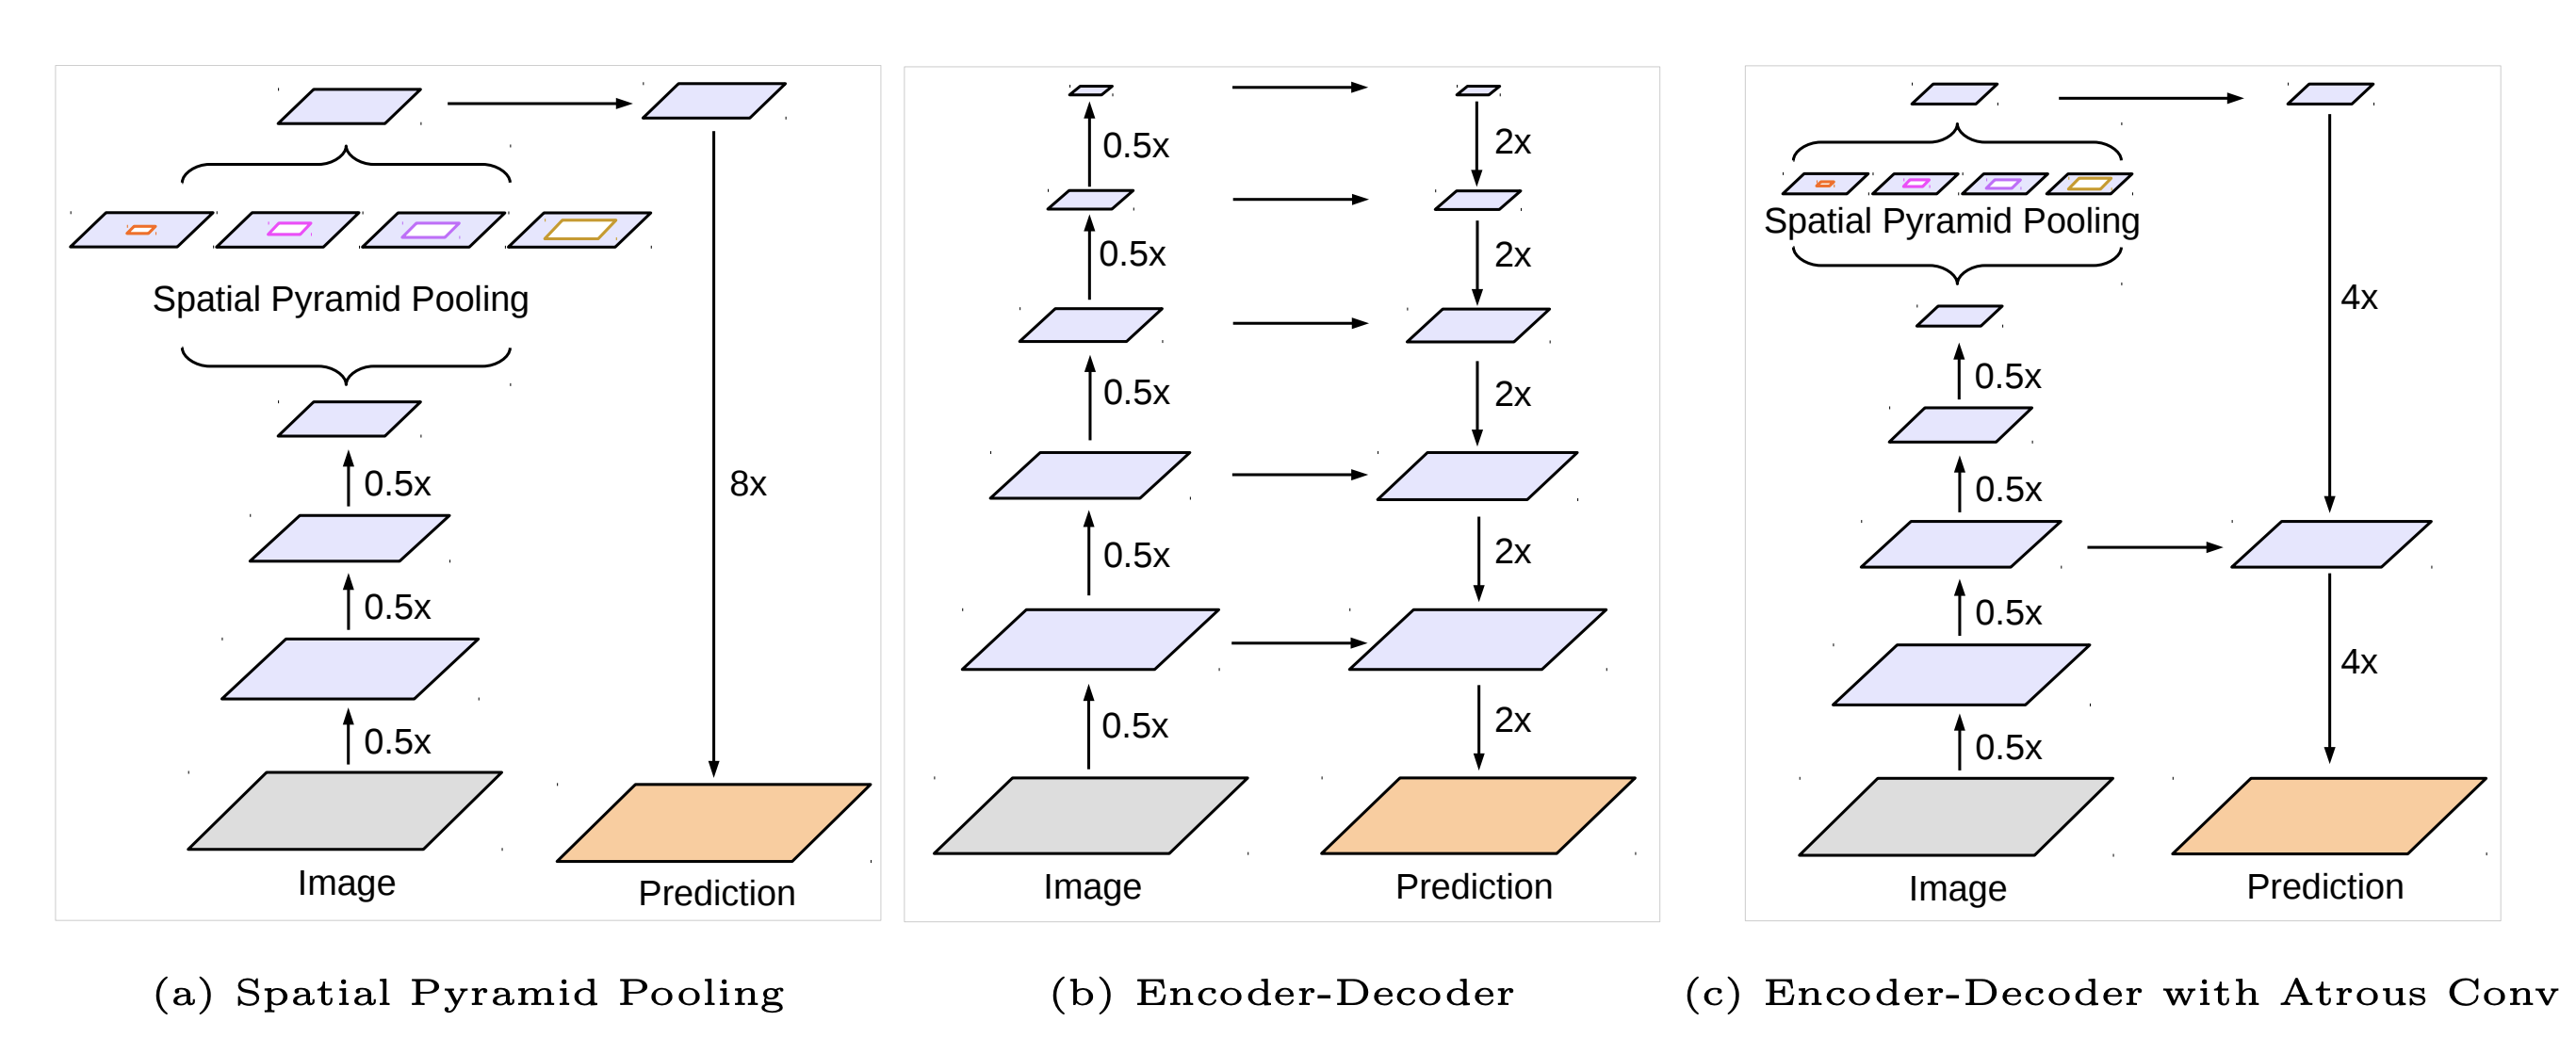
\includegraphics[width=0.9\textwidth]{figures/deeplab_encoderdecoder.png} %choose your uploaded image from folder "Images"
  \caption{The spatial pyramid pooling module of DeepLabv3 (a), the encoder-decoder structure (b) and DeepLabv3+ adaptation (c) \cite{chen2018encoder}} %figure caption
  \label{fig:deeplab} %labelling for internal reference
\end{figure} 
DeepLabv3+~\cite{chen2018encoder} adds the decoder module on top of the encoder output, as shown in Fig.~\ref*{fig:deeplabv3plus}.
In the decoder module, the 1$\times$1 convolution reduces the channels of the
low-level feature map from the encoder module which is then concatenated with the
DeepLabv3 feature map and the 3$\times$3 convolution obtains sharper segmentation results.
As a result, DeepLabv3+ holds rich semantic information from the encoder module,
while the detailed object boundaries are recovered by the decoder module and the spatial information is retrieved.
\begin{figure}[h] %h=here; t=top; b=bottom of the page
  \centering
  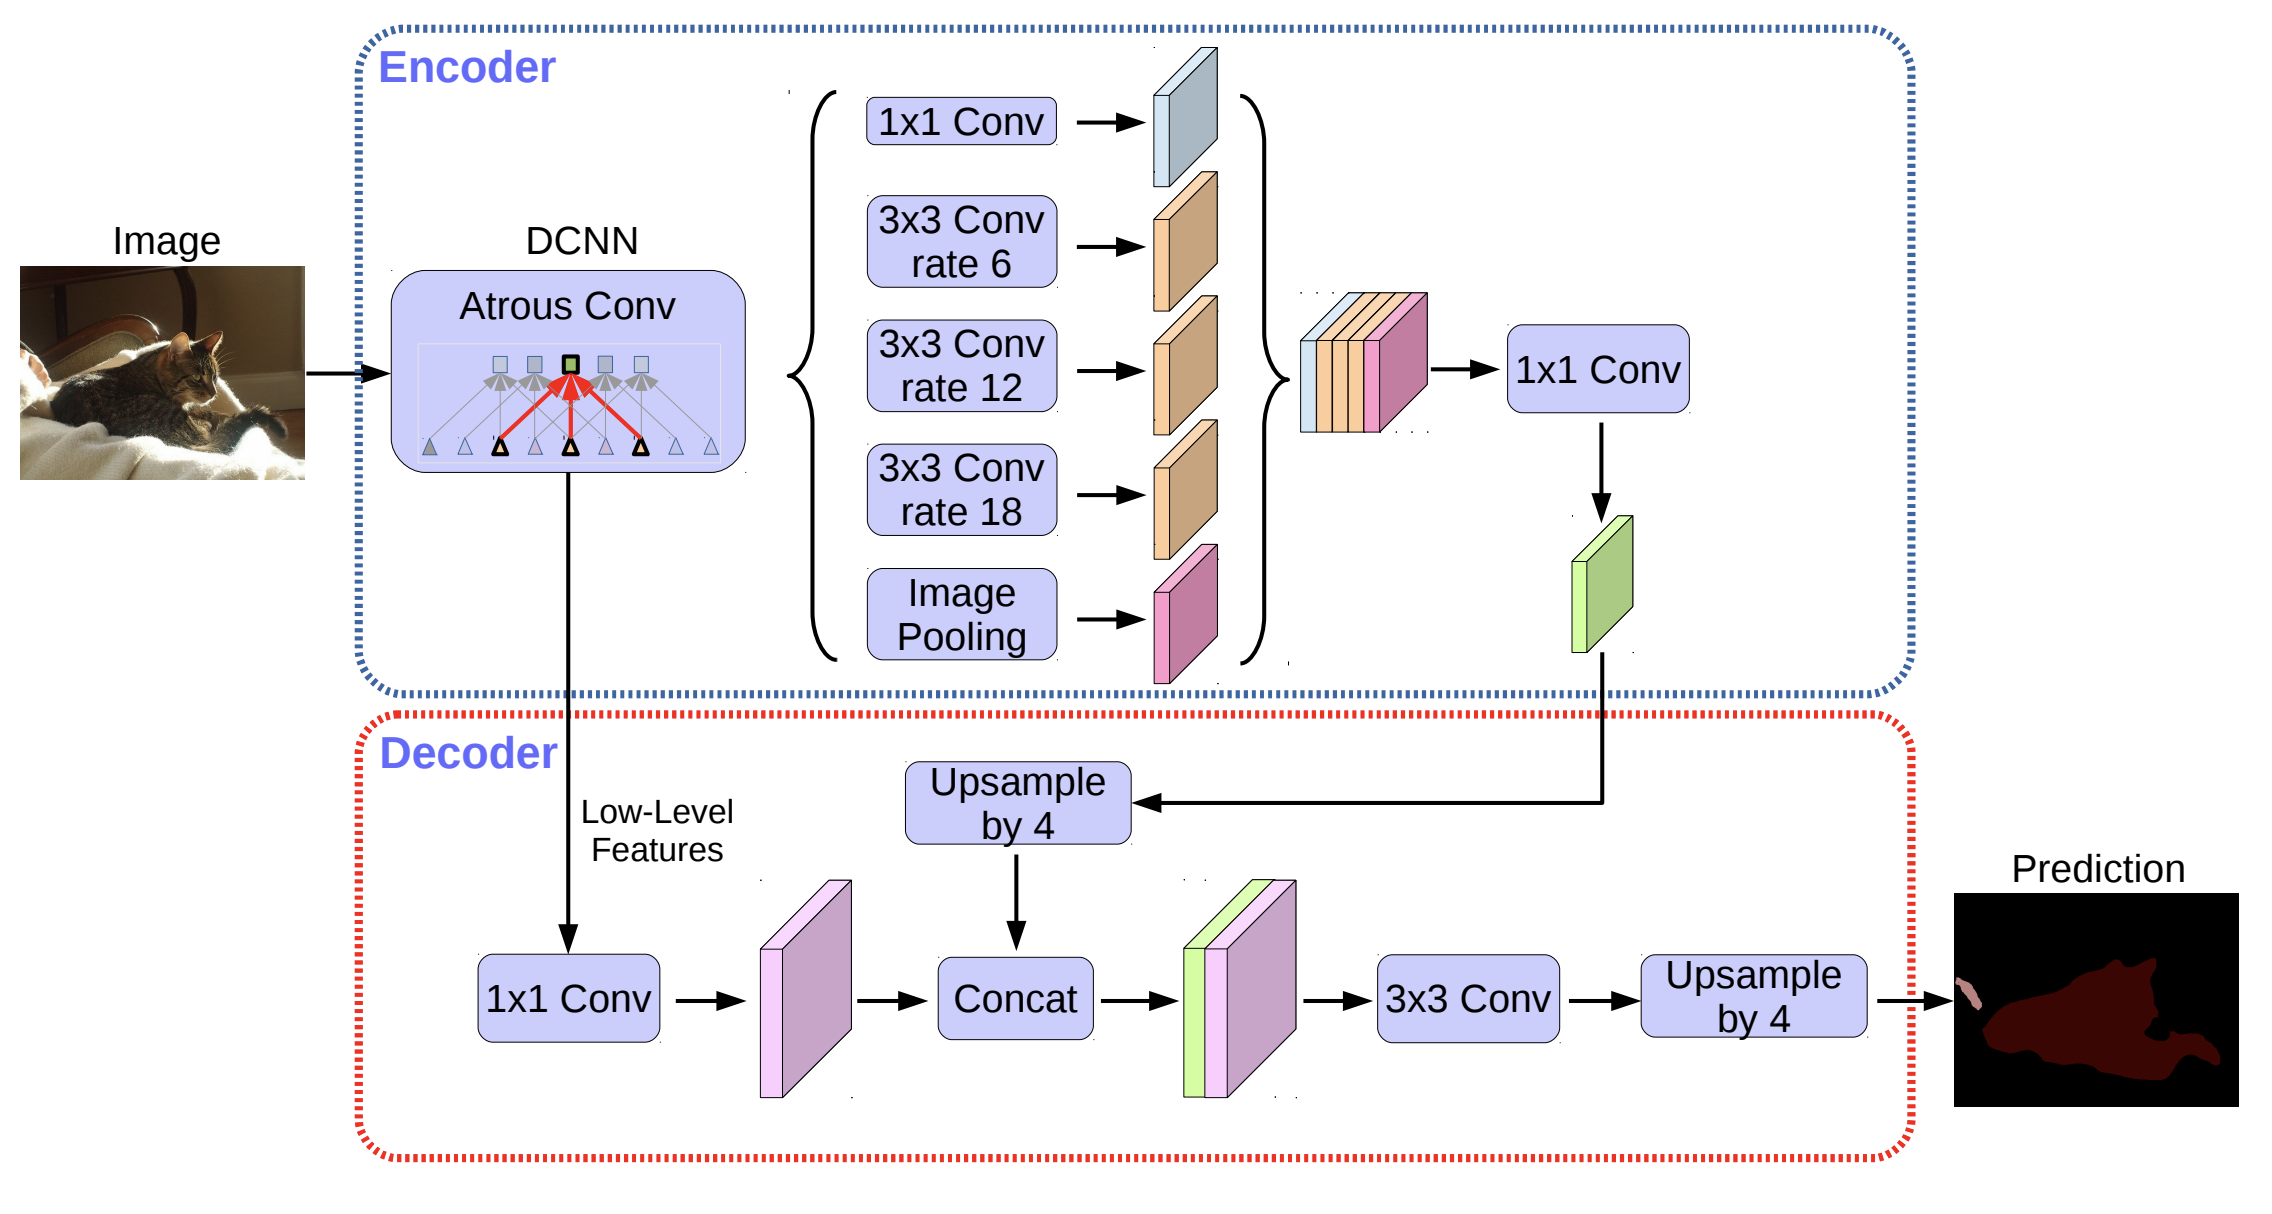
\includegraphics[width=0.9\textwidth]{figures/deeplabv3plus.png} %choose your uploaded image from folder "Images"
  \caption{DeepLabv3+ architecture. DeepLabv3 as encoder and proposed decoder structure for semantic image segmentation. \cite{chen2018encoder}} %figure caption
  \label{fig:deeplabv3plus} %labelling for internal reference
\end{figure} 

\subsection{Transformers}
Transformers~\cite{vaswani2017attention} were originally designed for the neural machine translation
problem in NLP to capture long-range dependencies among words in a sentence.
Their architecture converts one sequence into another one based on encoder-decoder architecture,
but it differs from the previously existing sequence-to-sequence models because
it does not imply any Recurrent Networks. 
\begin{wrapfigure}{r}{0.45\textwidth}
  \centering
  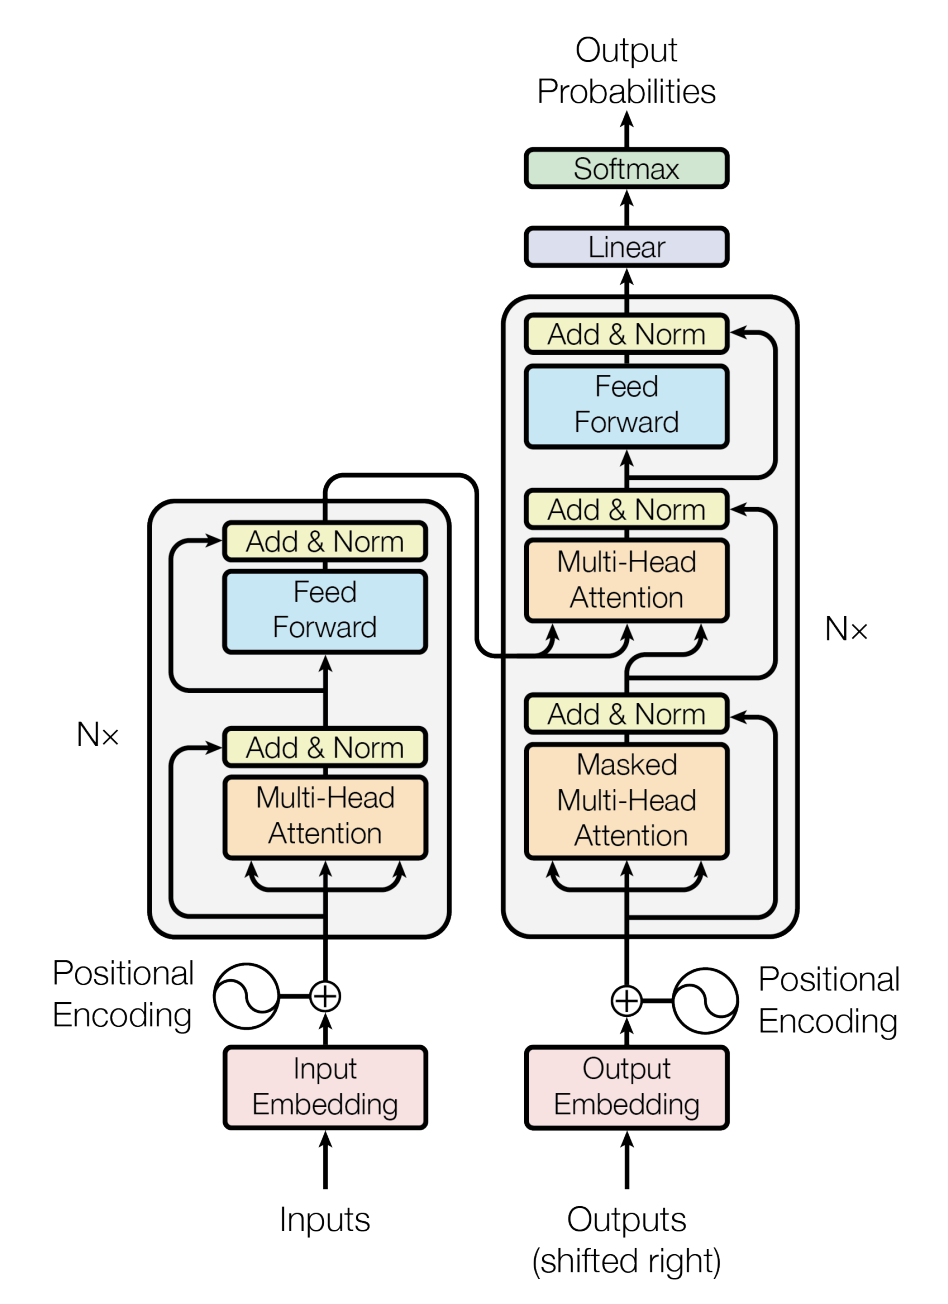
\includegraphics[width=0.4\textwidth]{figures/03_transformer_overview.png}
  \caption{Transformer model architecture. \cite{vaswani2017attention}}
  \label{fig:trans_arch}
\end{wrapfigure}
The input and output are first embedded into an $n$-dimensional space.
The following modules consist mainly of Multi-Head Attention and Feed Forward layers. 
Encoder (Figure~\ref{fig:trans_arch}, left) and decoder (Figure~\ref{fig:trans_arch}, right)
are composed of those modules that can be stacked on top of each other $N\times$ times.

Self-attention is a sequence-to-sequence operation.
It takes a weighted average over all the input vectors using dot product.
Scaled Dot-Product Attention (Figure~\ref{fig:trans_attn}, left) can be described by the following equation:
\begin{equation} \label{eq:1}
Attention(Q,K,V) = softmax(\frac{QK^T}{\sqrt{d_k}})V
\end{equation}
where $Q$ is a matrix of vector representation of one word in the sequence,
$K$ contains vector representations of all the words in the sequence and
$V$ contains again the vector representations of all the words in the sequence.
For the multi-head attention modules in the encoder and decoder,
$V$ consists of the same word sequence as $Q$.
However, for the attention module that is taken into account,
the encoder \underline{and} the decoder sequences, $V$ and $Q$ are different.
The Multi-Head Attention (Figure~\ref{fig:trans_attn}, right) concatenates multiple
attention outputs linearly to expected dimensions.
It can be parallelized into multiple mechanisms.
The attention mechanism is repeated multiple times with linear projections of $Q$, $K$, and $V$.
This allows the system to learn from different representations of $Q$, $K$, and $V$.
These linear representations are achieved by multiplying $Q$, $K$,
and $V$ by weight matrices that are learned during the training.

\begin{figure}[h] %h=here; t=top; b=bottom of the page
    \centering
    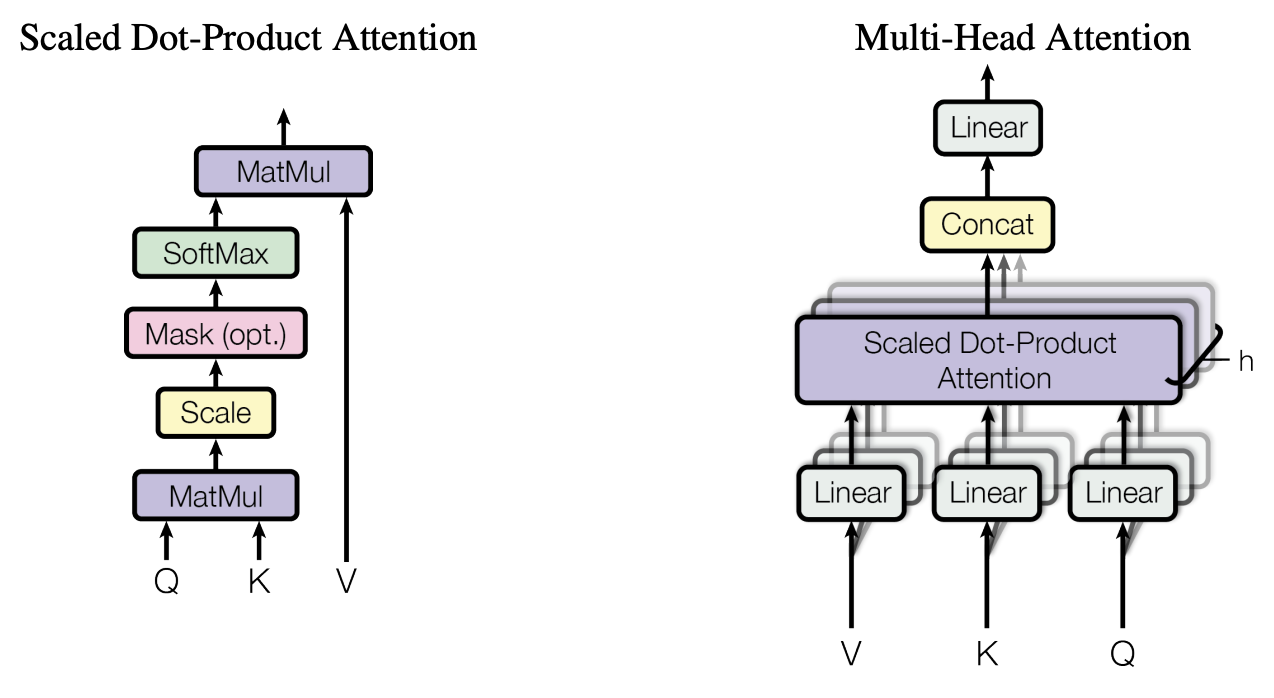
\includegraphics[width=0.7\textwidth]{figures/03_blocks_overview.png} %choose your uploaded image from folder "Images"
    \caption{Scaled Dot-Product Attention (left). Multi-Head Attention consists of several attention layers running in parallel (right). \cite{vaswani2017attention}} %figure caption
    \label{fig:trans_attn} %labelling for internal reference
\end{figure} 

This Feed-Forward layers can be described as a separate, identical linear transformation of each element from the given sequence. They have identical parameters for each position.

Naive application of transformers approach into the image domain would require evaluation of relations between each pixel and every other pixel, which is obviously not scalable. The Visual transformer (ViT) \cite{dosovitskiy2020image} is the first work to prove that a pure Transformer can achieve state-of-the-art performance in image classification. ViT converts the input image into a 1D series by cutting it into patches and feeding it to a linear layer. It yields a patch embedding. Position embeddings are added to the image patch embeddings. Adding the learnable position embeddings to each patch allows the model to learn the structure of the image. The rest of the pipeline is a standard encoder and decoder blocks of the transformer.  The decoder learns to map patch-level encodings coming from the encoder to patch-level class scores. Next, these patch-level class scores are upsampled by bilinear interpolation to pixel-level scores.

\subsubsection{SegFormer}
SegFormer~\cite{xie2021segformer} is a positional-encoding-free transformer based semantic segmentation method. As depicted in Figure \ref{fig:segformer_over}, it consists of two main modules: a hierarchical Transformer encoder to generate high-resolution coarse features and low-resolution fine features; and a lightweight All-MLP decoder to fuse these multi-level features to produce the final semantic segmentation mask. 

\begin{figure}[h] %h=here; t=top; b=bottom of the page
    \centering
    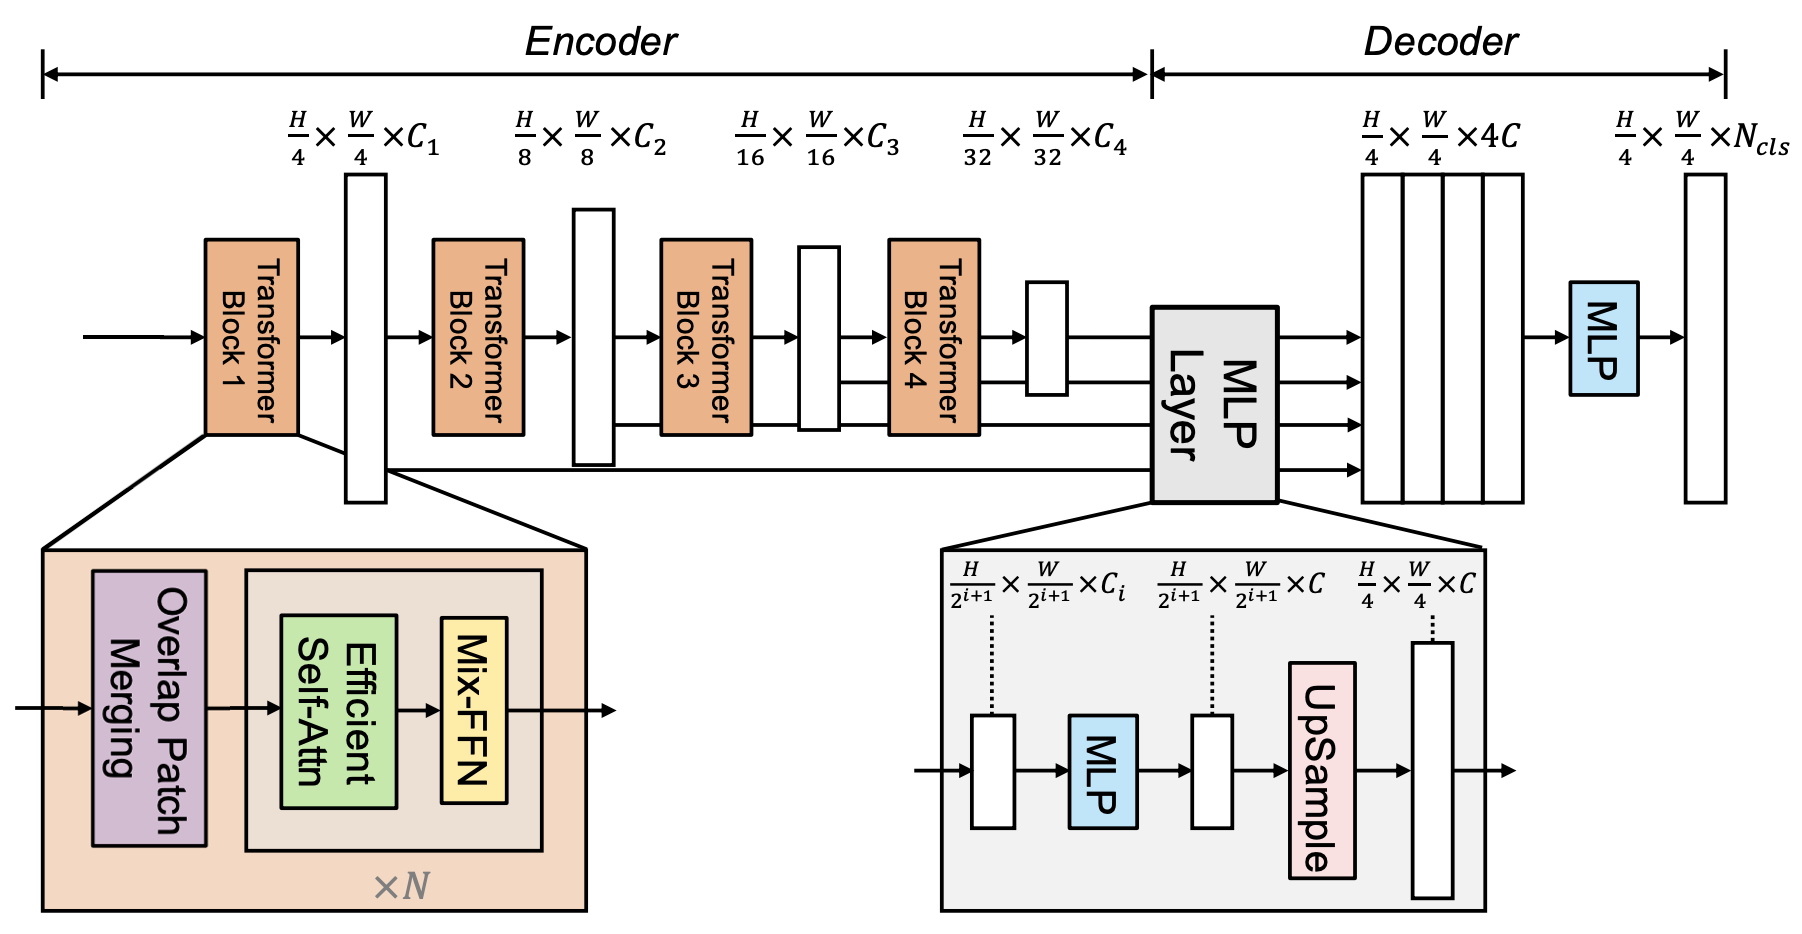
\includegraphics[height=60mm]{figures/03_segformer_overview.png} %choose your uploaded image from folder "Images"
    \caption{SegFormer consists of two main modules: A hierarchical Transformer encoder to extract coarse and fine features; and a lightweight All-MLP decoder to directly fuse these multi-level features and predict the semantic segmentation mask. “FFN” indicates feed-forward network. (modified image \cite{xie2021segformer} according to the official implementation)} %figure caption
    \label{fig:segformer_over} %labelling for internal reference
\end{figure} 

The $H\times W \times 3$ input image is divided into patches of size $4\times 4$. Those patches are forwarded to the hierarchical Transformer encoder to obtain multi-level features at $\frac{1}{4}, \frac{1}{8}, \frac{1}{16}, \frac{1}{32}$ resolution.

Overlapped Patch Merging produces features given an image patch and parameters: patch size $K$, stride between two adjacent patches $S$, and padding size $P$.

The main computation bottleneck of each transformer block in encoder is the self-attention layer. In SegFormer, before applying the self-attention according to the formula~\ref{eq:1}, the sequence $K$ is reduced by ratio $R$:
$$\hat{K} = Reshape(\frac{N}{R}, C\cdot R)(K)$$
$$K = Linear(C \cdot R, C)(\hat{K})$$
where $N = H \times W$, $Reshape(\frac{N}{R}, C \cdot R)(K)$ refers to reshaping $K$ to the the shape of $\frac{N}{R} \times (C \cdot R)$, and $Linear(C \cdot R, C)(\hat{K})$ refers to a linear layer taking a $(C \cdot R)$-dimensional tensor as input and generating a $C$-dimensional tensor as output. Therefore, the new $K$ has dimensions $\frac{N}{R} \times C$.  

Mix-FFN (feed-forward network) can be formulated as:
$$x_{out} = MLP(GELU(Conv 3\times 3(MLP(x_{in})))) + x_{in}$$
where $x_{in}$ is the feature from the self-attention module.

The multi-level features are then passed to All-MLP decoder to predict the segmentation mask at $\frac{H}{4}\times \frac{W}{4}\times N_{cls}$ resolution, where $N_{cls}$ is the number of classes.

The proposed All-MLP decoder consists of four main steps. First, multi-level features from
the encoder go through an MLP layer to unify the channel dimension (\ref{eq:2}). Then, features are up-sampled to $\frac{1}{4}$th of the original image (\ref{eq:3}). Third, a MLP layer is adopted to fuse the concatenated features (\ref{eq:4}). Finally, another MLP layer takes the fused feature to predict the segmentation mask (\ref{eq:5}).
\begin{equation} \label{eq:2}
\hat{F_i} = Linear(C_i, C)(F_i), \forall i
\end{equation}
\begin{equation} \label{eq:3}
\hat{F_i} = Upsample(\frac{H}{4}\times \frac{W}{4})(\hat{F_i}), \forall i
\end{equation}
\begin{equation} \label{eq:4}
F = Linear(4C, C)(Concat(\hat{F_i})), \forall i
\end{equation}
\begin{equation} \label{eq:5}
M = Linear(C, N_{cls})(F)
\end{equation}
where $F_i$ is the the feature and $M$ is the final mask.